	%
% Niniejszy plik stanowi przykład formatowania pracy magisterskiej na
% Wydziale MIM UW.  Szkielet użytych poleceń można wykorzystywać do
% woli, np. formatujac wlasna prace.
%
% Zawartosc merytoryczna stanowi oryginalnosiagniecie
% naukowosciowe Marcina Wolinskiego.  Wszelkie prawa zastrzeżone.
%
% Copyright (c) 2001 by Marcin Woliński <M.Wolinski@gust.org.pl>
% Poprawki spowodowane zmianami przepisów - Marcin Szczuka, 1.10.2004
% Poprawki spowodowane zmianami przepisow i ujednolicenie 
% - Seweryn Karłowicz, 05.05.2006
% Dodanie wielu autorów i tłumaczenia na angielski - Kuba Pochrybniak, 29.11.2016

% dodaj opcję [licencjacka] dla pracy licencjackiej
% dodaj opcję [en] dla wersji angielskiej (mogą być obie: [licencjacka,en])
\documentclass[licencjacka]{pracamgr}


% Dane magistrantów:
\autor{Maciej Góralski}{346144
\vspace{2em}}
\autori{Kacper Pawelec}{332436
\vspace{2em}}
\autorii{Aliaksei Suvorau}{374118}
\autoriii{Michał Swidziński}{371800}


% Dane magistrantów:
%\autor{Autor Zerowy}{342007}
%\autori{Autor Pierwszy}{342013}
%\autorii{Drugi Autor-Z-Rzędu}{231023}
%\autoriii{Trzeci z Autorów}{777321}
%\autoriv{Autor nr Cztery}{432145}
%\autorv{Autor nr Pięć}{342011}

\title{Zapisy na spotkania w systemie USOS}


%\tytulang{An implementation of a difference blabalizer based on the theory of $\sigma$ -- $\rho$ phetors}

%kierunek: 
% - matematyka, informacyka, ...
% - Mathematics, Computer Science, ...
\kierunek{informatyka}

% informatyka - nie okreslamy zakresu (opcja zakomentowana)
% matematyka - zakres moze pozostac nieokreslony,
% a jesli ma byc okreslony dla pracy mgr,
% to przyjmuje jedna z wartosci:
% {metod matematycznych w finansach}
% {metod matematycznych w ubezpieczeniach}
% {matematyki stosowanej}
% {nauczania matematyki}
% Dla pracy licencjackiej mamy natomiast
% mozliwosc wpisania takiej wartosci zakresu:
% {Jednoczesnych Studiow Ekonomiczno--Matematycznych}

% \zakres{Tu wpisac, jesli trzeba, jedna z opcji podanych wyzej}

% Praca wykonana pod kierunkiem:
% (podać tytuł/stopień imię i nazwisko opiekuna
% Instytut
% ew. Wydział ew. Uczelnia (jeżeli nie MIM UW))
\opiekun{dr Janina Mincer-Daszkiewicz\\
  Uniwersytet Warszawski\\
  }

% miesiąc i~rok:
\date{Grudzień 2018}

%Podać dziedzinę wg klasyfikacji Socrates-Erasmus:
\dziedzina{ 
%11.0 Matematyka, Informatyka:\\ 
%11.1 Matematyka\\ 
%11.2 Statystyka\\ 
11.3 Informatyka\\ 
%11.4 Sztuczna inteligencja\\ 
%11.5 Nauki aktuarialne\\
%11.9 Inne nauki matematyczne i informatyczne
}

%Klasyfikacja tematyczna wedlug AMS (matematyka) lub ACM (informatyka)
\klasyfikacja{Software and its engineering\\
Software creation and management\\
Software evolution\\}

% Słowa kluczowe:

\keywords{USOS, USOSadm, USOSweb, zapisy, spotkania, Dziekan, Sekcja Studencka}

% Tu jest dobre miejsce na Twoje własne makra i~środowiska:
\newtheorem{defi}{Definicja}[section]
\usepackage{hyperref}
\usepackage{enumitem}
\usepackage{calc}
\usepackage{tabularx}
\usepackage{array}
\usepackage{booktabs}
\usepackage[tableposition = top]{caption}
% \usepackage[none]{hyphenat}
\usepackage{graphicx}

\newlist{step}{enumerate}{10}
\setlist[step]{label*=\arabic*.,leftmargin=2em}
%\setlistdepth{10}

\newcolumntype{s}{>{\hsize=.35\hsize}X}
\newcolumntype{h}{>{\centering}X}
\newcolumntype{v}{>{\hsize=28px\centering\arraybackslash}X}
\newcolumntype{m}{>{\hsize=50px\centering\arraybackslash}X}
\newcolumntype{n}{>{\hsize=50px\arraybackslash}X}

% koniec definicji

\begin{document}

\maketitle

%tu idzie streszczenie na strone poczatkowa
\begin{abstract}
  Praca polega na dodaniu funkcjonalności do systemów USOSadm i USOSweb.
  Funkcjonalność ta umożliwi zdalną rejestrację zapisów do Dziekana dla studentów, co zaoszczędzi czasu, zmniejszy kolejki do Sekcji Studenckiej i pozwoli na zbieranie informacji do celów statystycznych.
  Ponadto zdalna rejestracja będzie dużo wygodniejsza zarówno dla Dziekana, pracowników Sekcji Studenckiej jak i studentów.
\end{abstract}

\tableofcontents
%\listoffigures
%\listoftables

\chapter{Wprowadzenie}
\section{Rozwiązanie dotychczasowe}
Obecnie student chcący zapisać się na spotkanie z Dziekanem musi przejść przez następujący proces:
\begin{enumerate}
\item Przyjść, zadzwonić albo wysłać e-mail do Sekcji Studenckiej.
\item Podać imię, nazwisko, numer indeksu oraz powód wizyty.
\item Student otrzymuję odpowiedź od Sekcji Studenckiej gdzie, w zależności od zasadności powodu, zawierającą numer jaki zajmuje on na liście. 
\end{enumerate}
W zależności od wybranej formy komunikacji oraz okresu w jakim student się zapisuje, czas oczekiwania może być istotnie długi. Momentem gdy szczególnie trudno jest uzyskać kontakt z~Sekcją~Studencką jest okres przedłużania ważności legitymacji studenckich. Wtedy kolejki studentów potrafią być na tyle długie że w rozsądnym czasie student niekoniecznie będzie mógł wejść do~sekretariatu, co jest najpewniejszą formą zapisania się.

Kluczowy jest tutaj fakt, że Sekcja Studencka na Wydziale MIM otwarta jest dla studentów tylko w poniedziałki, wtorki, czwartki i~piątki przez okres 3 godzin dziennie. Ogranicza to czasowe możliwości studentów na zapisy. Co więcej, forma w jakiej przebiegają zapisy niepotrzebnie zajmuje czas studentów i~pracowników Sekcji Studenckiej.


\section{Ogólnie informacje o systemie USOS}
\href{http://usos.edu.pl}{USOS}, czyli Uniwersytecki System Obsługi Studiów, powstał w~wyniku zapotrzebowania na~narzędzie~informatyczne służące do~zarządzania sprawami studiów na~polskich~uczelniach. Razem z~sukcesem USOS powstała potrzeba żeby stworzyć platformę umożliwiającą studentom częściowy dostęp do możliwości jakie dostarcza USOS --- w tym celu powstał \href{htpp://usosweb.uw.edu.pl}{USOSweb}. Internetowa platforma pozwalająca studentom i pracownikom uczelni na dostęp do i~pozwalająca na częściową modyfikację danych z USOS.

USOS dostarcza takie usługi jak:
\begin{enumerate}
\item Rekrutacja na studia i~immatrykulacja.
\item Elektroniczne Legitymacje Studenckie.
\item Przygotowywanie oferty dydaktycznej. 
\item Zarządzanie tokiem studiów.
\item Podania, stypendia i~ankiety.
\item Akademiki i~płatności
\end{enumerate}
oraz inne.

\section{Cel pracy}
W ramach pracy powstał moduł do systemów USOSadm i~USOSweb, dzięki któremu będzie możliwe tworzenie, kontrola i~archiwizacja wizyt studentów u~Dziekana. W USOSweb studenci i~osoby spoza wydziału będą mogły zapisywać się na spotkania z~Dziekanem w~odgórnie ustalonych terminach. Poza ułatwieniem rejestracji i~zwiększeniem jej dostępności, system ten będzie również maksymalizować wykorzystanie czasu Dziekana oraz studentów.
\section{Struktura pracy}
Praca składa się z~6 rozdziałów i~dodatków.
Uwagi i~wymagania potencjalnych użytkowników zostały opisane w~rozdziale~\ref{chap:wymagania}.
W~rozdziale~\ref{chap:specyfikacja} znajduje się specyfikacja nowych funkcjonalności. W~rozdziale \ref{chap:implementacja} jest zawarty opis technologii użytych do~implementacji oraz jej szczegóły. Potencjalny rozwój nowego modułu jest opisany w~rozdziale \ref{chap:rozwoj}, a dokumentacje dotyczące naszej funkcjonalności są w~rozdziale~\ref{chap:dodatki}. 

\section{Podział pracy}
Podział pracy w projekcie wygląda następująco:
\begin{itemize}
\setlength\itemsep{0,05em}
\item Maciej Góralski --- praca nad USOSadm w Java oraz pisanie pracy   licencjackiej,
\item Kacper Pawelec --- praca nad USOSadm w Java,
\item Aliaksei Suvorau --- praca nad USOSweb w PHP i MySQL,
\item Michał Swidziński --- praca nad USOSadm w Java.
\end{itemize}


\chapter{Wymagania użytkowników} \label{chap:wymagania}

\section{Wymagania}
Przed przystąpieniem do projektowania systemu postanowiliśmy zapytać potencjalnych użytkowników jakie mają wymagania względem systemu. Zidentyfikowaliśmy trzy główne grupy użytkowników które zapytaliśmy o zdanie: Dziekana, studentów oraz~pracowników Sekcji Studenckiej Dziekanatu.

\section{Rozmowa z Dziekanem}
Dziekana, będącego jednym z głównych odbiorców modułu, jako pierwszego zapytaliśmy o~wymagania względem projektu. Najistotniejsze z~nich to:

\begin{itemize}
\setlength\itemsep{0,05em}
\item Powinien istnieć mechanizm ręcznej i automatycznej akceptacji próśb o spotkanie.
\item Moduł musi dawać możliwość konfiguracji limitów czasowych oraz limitów ilości osób.
\item Jednocześnie można być zapisanym tylko na jedno spotkanie.
\item Dziekan powinien mieć możliwość zostawienia w systemie notatki ze~spotkania.
\item Powinno być możliwe usuwanie informacji o starych spotkaniach, z zachowaniem notatek.
\end{itemize}
Wymagania jakie przedstawił Dziekan w dużej mierze uformowały kształt jaki ten projekt przyjął. Na ich podstawie rozwijaliśmy lub~dodawaliśmy do modułu funkcjonalności.

\section{Ankieta dla studentów}
W trakcie projektowania modułu przeprowadziliśmy ankietę wśród studentów aby dowiedzieć się jakie byłyby ich preferencje względem niektórych funkcjonalności i~czy pokrywają się z~wymyślonymi przez nas rozwiązaniami. Ich odpowiedzi wyglądały następująco:
\begin{itemize}
\setlength\itemsep{0,05em}
\item Jak wcześnie przed wizytą chciałbyś/chciałabyś zapisać się do dziekana?
\begin{itemize}
\setlength\itemsep{0,05em}
\item Tego samego dnia --- 28.2\%.
\item Na tydzień przed --- 66.47\%.
\item Na dwa tygodnie przed --- 2.94\%.
\item Na trzy tygodnie przed --- 0.00\%.
\item Na miesiąc przed --- 1.76\%.
\item Na dłużej niż miesiąc przed --- 0.00\%.
\end{itemize}

\item W wypadku gdy limit dostępnych miejsc się zapełni, chciałbyś/chciałabyś:
\begin{itemize}
\setlength\itemsep{0,05em}
\item Zostać zapisanym/zapisaną na najbliższy dostępny termin --- 10\%.
\item Zostać zapisanym na następny termin wyznaczony przez siebie --- 79.41\%.
\item Nic, chcę zapisać się od nowa samodzielnie --- 10.59\%.
\end{itemize}

\item Podając powód na wizytę u Dziekana, chcę:
\begin{itemize}
\setlength\itemsep{0,05em}

\item Napisać powód samemu - 6.47\%.
\item Wybrać powód z listy dostępnych możliwych powodów - 9.41\%.
\item Mieszankę powyższych odpowiedzi - 84.12\%.
\end{itemize}

\item Czy zapisując się do Dziekana bierzesz pod uwagę możliwość w której nie będziesz w stanie pojawić się na wizycie wiedząc, że to może grozić trudnościami przy kolejnych zapisach? Jeśli tak, to jak sobie wyobrażasz optymalny system zapisów? Wszelkie inne uwagi podaj również w tym polu.
\begin{itemize}
\setlength\itemsep{0,05em}
\item ``Chcę móc odwołać bez podania powodu``
\item ``Zazwyczaj z powodu nagłych wypadków / choroby - 1-4 dni przed / rano tego samego dnia``
\item ``wypadki losowe, 2-3 dni przed``
\item ``24h brzmi sensownie``
\end{itemize}

\end{itemize}
Większość studentów potwierdziła, że zaprojektowane przez nas rozwiązanie będzie dla nich wygodne i~funkcjonalne.
 
\section{Rozmowa z Sekcją Studencką}
Zapytaliśmy o zdanie również pracowników Sekcji Studenckiej. Ich wymagania wyglądały następująco:
\begin{itemize}
\setlength\itemsep{0,05em}
    \item System powinien być wygodny i prosty w obsłudze.
    \item Jak najwięcej opcji i pól powinno mieć domyślne wartości.
    \item Powinna istnieć opcja automatycznej akceptacji spotkań.
    \item Limity dostępnych miejsc, czasowe i inne powinny być modyfikowalne.
\end{itemize}
Odpowiedź pracowników Sekcji Studenckiej wyraźnie podkreśliła wagę jaką ma wygoda i~łatwość użytkowania. W związku z tym w postanowiliśmy położyć dodatkowy nacisk na~te~cechy systemu.


\chapter{Specyfikacja} \label{chap:specyfikacja}

\section{Cel projektu}
Celem projektu jest dodanie do aplikacji USOSadm i USOSweb funkcjonalności zapisów na~spotkania z~Dziekanem. System dzieli się na dwie części: moduł USOSweb dla osoby zapisującej się na spotkanie i~moduł USOSadm dla personelu obsługującego spotkania.
 
\section{Zapisy}
Zapisy na spotkania będą realizowane poprzez kalendarz spotkań, ich przebieg będzie wyglądał następująco:

\begin{itemize}
    \item Zdefiniowanie terminu spotkania.
    \item Okres zapisów: interesanci składają prośby o spotkanie w~formie formularzy.
    \item Okres akceptacji: pracownicy przeglądają formularze i akceptują lub odrzucają prośby.
    \item Spotkanie odbywa się.
\end{itemize}

\section{Cykl zapisów}
W cyklu zapisów można wyróżnić następujące kluczowe informacje:

\begin{itemize}
\setlength\itemsep{0,05em}
    \item Data i godzina spotkania .
    \item Termin początku i końca okresu zapisów.
    \item Termin początku i końca okresu akceptacji.
    \item Limit miejsc na spotkanie.
    \item Limit miejsc rezerwowych na spotkanie.
    \item Jednostkę, której dotyczy spotkanie.
    \item Osobę, której dotyczy spotkanie
\end{itemize}

Porządek chronologiczny terminów:

\begin{itemize}
\setlength\itemsep{0,05em}
    \item Początek okresu zapisów.
    \item Koniec okresu zapisów.
    \item Początek okresu akceptacji.
    \item Koniec okresu akceptacji.
    \item Termin spotkania.
\end{itemize}

\section{Dodatkowe wymagania}
Interesanci po zapisaniu się na~spotkanie mogą zostać zaakceptowani, odrzuceni lub mogą nie zmieścić się w~limicie miejsc. Ci, którzy nie zmieścili się~w~limicie, mają przez ograniczony czas możliwość przepisania swojego spotkania na~inny~termin, na~który zapisy nie zostały jeszcze otwarte. Odrzuceni interesanci nie mają takiej możliwości.

Limit miejsc rezerwowych ma służyć maksymalnemu wykorzystaniu czasu na~spotkania. W przypadku gdy osoba potwierdzająca zapisy studenta odrzuci jego prośbę o~spotkanie z Dziekanem, zostanie ona usunięta z~kolejki, wszyscy studenci niżej na~liście głównej przeniesieni o~jedno miejsce wyżej i, jeśli ktoś się na niej znajduje, pierwsze miejsce na~liście~rezerwowej zostanie przeniesione na~listę~główną.


\section{Formularz}
Formularz zapisów zawiera następujące informacje:

\begin{itemize}
\setlength\itemsep{0,05em}
    \item Imię i nazwisko osoby zapisującej się.
    \item Numer indeksu, jeśli jest studentem.
    \item Powód spotkania.
    \item Spotkanie, którego dotyczy formularz.
    \item Czy formularz jest “nowy” w aktualnym cyklu zapisów.
    \item Informacja czy spotkanie zostało zaakceptowane, odrzucone czy~nierozpatrzone.
    \item Informacja czy spotkanie się odbyło.
    \item Uzasadnienie odrzucenia.
\end{itemize}
Status “nowości” formularz zyskuje w~chwili utworzenia. Tracony jest podczas pierwszego przeglądania przez personel. Służy szybkiemu docieraniu do~nowych formularzy, w przypadku wielokrotnego przeglądania.

\section{Szczegółowa specyfikacja użytkowania}

\subsection{Używanie USOSadm poprzez już zalogowanego użytkownika z odpowiednimi uprawnieniami.}
	\begin{step}
		\item Utworzenie kalendarza spotkań.
			\begin{step}
				\item Podanie danych nowego kalendarza:
					\begin{itemize}
						\item Nazwa kalendarza.
						\item Cykl dydaktyczny.
						\item Jednostka w której odbywa się spotkanie.
						\item Osoba z którą odbywa się spotkanie.
					\end{itemize} 
				\item Załadowanie danych z już istniejącego kalendarza.
			\end{step}
				\item Utworzenie spotkań, dla każdego podanie:
					\begin{itemize}
						\item Początek i~koniec okresu zapisów.
						\item Początek i~koniec spotkania.
						\item Początek i~koniec okresu akceptacji.
					\end{itemize}
				\item Utworzenie listy powodów odrzuceń, dla każdego podając:
					\begin{itemize}
						\item Jednostkę organizacyjną.
						\item Nazwę.
						\item Treść powodu.
					\end{itemize}
		\item Udostępnienie kalendarza poprzez zmianę stanu na~"Dostępne".
		\item Okres akceptacji.
			\begin{step}
				\item Wyświetlenie list studentów.
					\begin{step}
						\item Sortowanie listy po:
							\begin{itemize}
								\item Imieniu.
								\item Nazwisku.
								\item Peselu.
								\item Indeksie.
						 	\end{itemize}
					\end{step}
				\item Akceptacja studenta.
				\item Odrzucenie studenta. 
			\end{step}
	\end{step}
	
\subsection{Używanie USOSweb poprzez już zalogowanego użytkownika z odpowiednimi uprawnieniami.}
	\begin{step}
			\item Wejście w widok "Dla studentów".
			\item Przejście w zakładkę "Moje jednostki lub~"Wszystkie jednostki".
			\item Wybranie jednostki, z możliwością sortowania po:
				\begin{itemize}
					\item Kodzie jednostki.
					\item Nazwie jednostki.
					\item Liczbie dostępnych spotkań. 
				\end{itemize}
			\item Przeglądanie dostępnych spotkań wybranej jednostki:
				\begin{step}
					\item Możliwość przeglądania nieaktywnych terminów z dostępnych spotkań.
					\item Dostęp do informacji o:
						\begin{itemize}
							\item Dacie spotkania.
							\item Godzinach w jakich odbywa się~spotkanie
							\item Początku i~końcu okresu zapisów.
							\item Stanie zapisów.
							\item Ilości zajętych miejsc.
						\end{itemize}
				\end{step}
			\item Zapisanie na spotkanie:
				\begin{step}
					\item Wybór spotkania.
					\item Wybranie powodu z listy dostępnych powodów.
					\item Wypełnienie pisemnego powodu.
				\end{step}
			\item Przeglądanie spotkań w zakładce "Moje spotkania"
				\begin{step}
					\item Możliwość sortowania po:
						\begin{itemize}
							\item Opisie spotkania.
							\item Kodzie jednostki.
							\item Dacie spotkania.
							\item Stanie zapisu:
								\begin{itemize}
									\item A -- zaakceptowane.
									\item N -- nierozpatrzone.
									\item O -- odrzucone.
								\end{itemize}
						\end{itemize}
				\end{step}
			\item Wypisanie ze spotkania:
				\begin{step}
					\item Znalezienie spotkania.
					\item Kliknięcie koszyka wypisania.
					\item Potwierdzenie decyzji.
				\end{step}
	\end{step}
	

\section{Dodatkowe wymagania}
	\begin{step}
		\item Interfejs powinien mieć zintegrowane, zrozumiałe instrukcje użytkowania.
		\item Interesanci nie mogą mieć dostępu do danych zapisów innych interesantów.
		\item Korzystanie z aplikacji wymaga konta w uczelnianym Centralnym Systemie Uwierzytelniającym (CAS, z ang. Central Authentication Service).
	\end{step}
	
\section{Schemat bazy danych}

\begin{figure}[b!]
  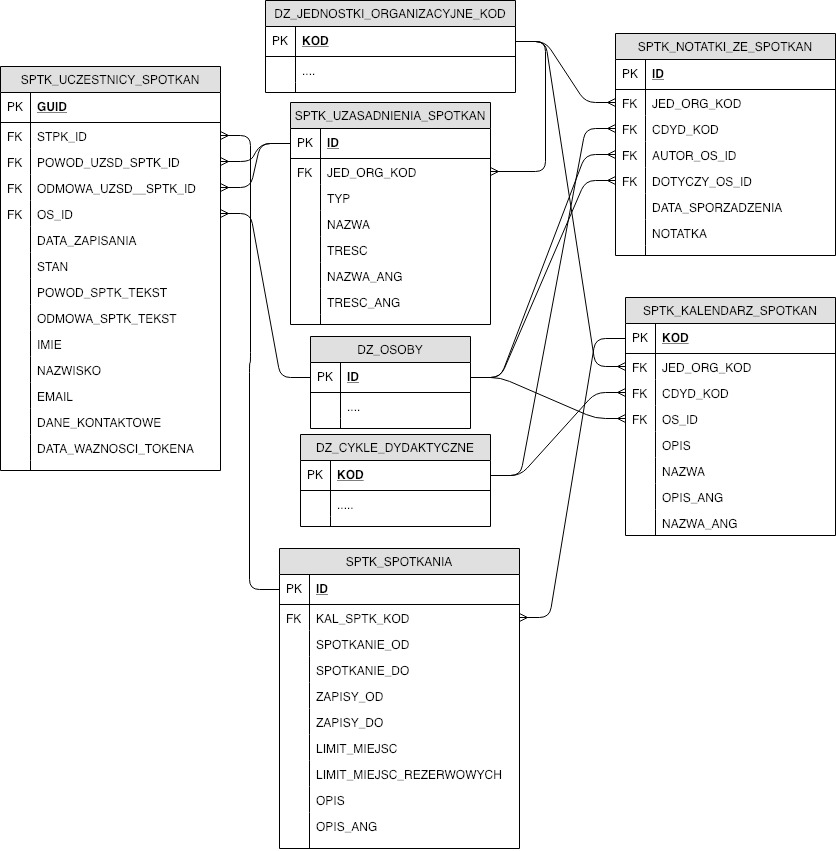
\includegraphics[width=\linewidth]{schemat.jpg}
  \caption{Schemat bazy danych.}
  \label{fig:schemat}
\end{figure}

W wyniku wymagań i potrzeb implementacyjnych, utworzyliśmy następujący schemat bazy danych, pokazany w obrazie \ref{fig:schemat}. Kluczowe jej tabele mają następujący skład:

\begin{itemize}
\item SPTK\textunderscore UCZESTNICY\textunderscore SPOTKAN
	\begin{itemize}
	\item Podstawowych danych uczestników spotkania.
	\item Id spotkania.
	\item Powód wraz z uzasadnieniem.
	\item Odmowę wraz z uzasadnieniem.
	\item Stan spotkania.
	\end{itemize}
\item SPTK\textunderscore SPOTKANIA
	\begin{itemize}
	\item Kalendarza spotkań.
	\item Dat spotkania i zapisów.
	\item Limitów miejsc.
	\item Opisu.
	\end{itemize}
\item SPTK\textunderscore NOTATKI\textunderscore ZE\textunderscore SPOTKAN
	\begin{itemize}
	\item Jednostki organizacyjnej.
	\item Cyklu dydaktycznego.
	\item Autora.
	\item Osoby której dotyczy.
	\item Daty utworzenia.
	\item Notatki.
	\end{itemize}
\end{itemize}


\section{Przykłady}
Przykładowe scenariusze użycia modułu. Dla prostoty przyjęto dzień jako niepodzielną jednostkę czasu.

%\begin{step}
%	\item Lista rezerwowa
	\setlength{\tabcolsep}{8pt}
	
\begin{table}[h]
	\begin{center}
	\centering
	\caption{Lista Rezerwowa}
	\begin{tabularx}{\textwidth}{ v X n }
	\toprule
	Dzień & Student & Spotkanie1 \\
	\midrule
	1  &    & Definicja \\
	\midrule[0.001em]
	2  & Dostępne spotkania: Spotkanie1.\newline Zapisanie na Spotkanie1, miejsce na~liście rezerwowej. & Zapisy \\
	\midrule[0.001em]
	3  & Kilka miejsc w kolejce zostaje zwolnionych, dostaje się na spotkanie  & Akceptacja \\
	\midrule[0.001em]
	4  &   & Spotkanie \\
	\bottomrule
	\end{tabularx}
	\end{center}
\end{table}
	
%\item Token przeniesienia
\begin{table}[h]
	\begin{center}
	\centering
	\caption{Token przenies	ienia}
	\begin{tabularx}{\columnwidth}{ v X n n }
	\toprule
	Dzień & Student & Spotkanie1 & Spotkanie2\\
	\midrule
	1  &    & Definicja & Definicja \\
	\midrule[0.001em]
	2  & Dostępne spotkania: Spotkanie1. \newline Zapisanie na Spotkanie1, miejsce na liście rezerwowej & Zapisy & \\
	\midrule[0.001em]
	3  & Nie dostaje się na spotkanie, pozostaje w rezerwie.  & Akceptacja & \\
	\midrule[0.001em]
	4  & Dostaje token przeniesienia. \newline Dostępne spotkania: Spotkanie2. \newline Przenosi się na Spotkanie2 & Spotkanie & \\
	\midrule[0.001em]
	5  &  &  & Zapisy\\
	\midrule[0.001em]
	6  & Dostaje się na spotkanie &  & Akceptacja\\
	\midrule[0.001em]
	7  &  &  & Spotkanie\\
	\bottomrule
	\end{tabularx}
	\end{center}
\end{table}
	
%\item Token przeniesienia pozwala na przeniesienie tylko do nierozpoczętej rejestracji
\begin{table}[h]
	\begin{center}
	\centering
	\caption{Token przeniesienia pozwala na przeniesienie tylko do nieotwartego spotkania}
	\begin{tabularx}{\columnwidth}{ v X n n n }
	\toprule
	Dzień & Student & Spotkanie1 & Spotkanie2 & Spotkanie3\\
	\midrule
	1  &    & Definicja & Definicja &\\
	\midrule[0.001em]
	2  & Dostępne spotkania: Spotkanie1. \newline Zapisanie na Spotkanie1, miejsce na liście rezerwowej. & Zapisy &  &\\
	\midrule[0.001em]
	3  & Nie dostaje się na spotkanie, pozostaje w rezerwie.  & Akceptacja &  &\\
	\midrule[0.001em]
	4  & Dostaje token przeniesienia.\newline Dostępne spotkania: brak & Spotkanie &  &\\
	\midrule[0.001em]
	5  & Token wygasa &  & Zapisy & Definicja\\
	\midrule[0.001em]
	6  &  &  & Akceptacja & Zapisy\\
	\bottomrule
	\end{tabularx}
	\end{center}
\end{table}
	
	\newpage
%\item Wiele tur jednocześnie
\begin{table}[h]
	\begin{center}
	\centering
	\caption{Wiele tur jednocześnie}
	\begin{tabularx}{\columnwidth}{ v X m m }
	\toprule
	Dzień & Student & Spotkanie1 & Spotkanie2 \\
	\midrule
	1  &    & Definicja & Definicja \\
	\midrule[0.001em]
	2  & Dostępne spotkania: Spotkanie1. \newline Zapisanie na Spotkanie1, miejsce na liście rezerwowej. & Zapisy & Zapisy\\
	\midrule[0.001em]
	3  & Nie dostaje się na spotkanie, pozostaje w rezerwie.  & Akceptacja & Zapisy\\
	\midrule[0.001em]
	4  & Dostaje token przeniesienia.\newline Dostępne spotkania: brak.\newline Dostępne spotkania: Spotkanie2.\newline Zapisanie na Spotkanie2 & Spotkanie & Zapisy\\
	\midrule[0.001em]
	5  & Token wygasa &  & Akceptacja \\
	\midrule[0.001em]
	6  &  &  & Spotkanie \\
	\bottomrule
	
	\end{tabularx}
	\end{center}
\end{table}
%\end{step}

\chapter{Implementacja} \label{chap:implementacja}
\section{USOS}
USOS jest skomplikowanym systemem, powstającym przez lata. Składa się on aktualnie z wielu komponentów odpowiadających za różne zbiory funkcjonalności potrzebnych do obsługi studiów. Ze względu na zróżnicowane okresy powstawania oraz przeznaczenie, różnią się między sobą znacząco technologią wykonania, a zasada współdziałania całego systemu jest bardzo skomplikowana.
Składowe, z którymi mieliśmy styczność podczas naszej pracy, to:
\begin{itemize}
\item USOSadm w Javie -- moduł przeznaczony dla pracowników administracji, pozwalający na cyfryzację typowych zadań administracyjnych, jak zarządzanie rejestracjami, płatnościami, wymianą międzynarodową etc.
\item USOSWeb -- moduł przeznaczony dla studentów napisany w PHP. Udostępnia podstawowe informacje o~toku~studiów studenta oraz~funkcje~zdalnego załatwiania wielu formalności, jak rejestracja na przedmioty czy składanie podań.
\item Baza danych Oracle -- centralna baza danych USOS. Posiada bogatą wewnętrzną logikę odpowiadającą między innymi za dostęp do danych. Bezpośrednio kontaktuje się z nią USOSadm.
\item Baza danych MySQL -- Baza danych z którą łączy się USOSWeb.
\item Migrator -- moduł odpowiedzialny za synchronizację baz danych. Ponieważ ruch w systemie USOS jest rozproszony pomiędzy wiele modułów i baz danych, Migrator dba o zachowanie spójności danych z centralną bazą wykonując częste, okresowe migracje.
\end{itemize}

\section{USOSadm} \label{sec:impusos}

\subsection{Informacje ogólne}
Celem prac w obrębie USOSadm było zaimplementowanie funkcjonalności przy wykorzystaniu przyjętych praktyk programistycznych. Jej zakres obejmował następujące mechanizmy:
\begin{itemize}
\item Definiowania nowych kalendarzy spotkań oraz spotkań z pracownikami uczelni.
\item Zapisu i akceptowania zapisów na spotkania studentów.
\item Sporządzania notatek ze spotkań.
\item Definiowania listy najczęstszych powodów zapisów na spotkania.
\item Mechanizm tokenowy, pozwalający odrzuconym studentom zapisać się na kolejne spotkanie z uprzywilejowaną pozycją.
\end{itemize}

\subsection{Aplikacja kliencka}
Aplikacja kliencka USOSadm to część aplikacji wykonywana po stronie klienta. Składa się m.in. z~kodu HTML i~skryptów JavaScript. Napisana została przy pomocy frameworka JavaServer Faces z wykorzystaniem biblioteki komponentów RichFaces.

\subsection{Serwer}
Serwer USOSadm odpowiedzialny jest za~większą część logiki aplikacji. Napisany został w Javie. Część logiki wykonywana jest po~stronie~bazy~danych~Oracle.

\subsection{Komunikacja z bazą danych}
Komunikacja z~bazą~danych została zrealizowana przy pomocy własnego, bogatego API zrealizowanego przy pomocy technologi Hibernate. Technologia Hibernate pozwala na~odwzorowanie danych z~bazy~danych za~pomocą odpowiednio spreparowanych obiektów w~Javie.

\subsection{Opis implementacji}
Funkcjonalność została wydzielona w oddzielnym module do USOSadm, "Spotkania". Składa się łącznie z 4 widoków:
\begin{itemize}
\item Słownik uzasadnień -- pozwala zdefiniować najczęstsze uzasadnienia zapisów na spotkania jak i odrzucenia spotkań.
\item Kalendarz Spotkań -- pozwala na definicję kalendarzy spotkań, spotkań, zapisywanie studentów oraz akceptowanie zapisów na spotkania.
\item Notatki -- pozwala na przeglądanie notatek ze spotkań osób oraz dodawanie nowych.
\item Spotkania osób -- udostępnia funkcjonalność potrzebną do przeprowadzenia spotkania, taką jak przeglądanie spotkań danej osoby, przeglądanie zapisów na spotkanie oraz notatek z poprzednich spotkań danej osoby.
\end{itemize}

\subsection{Słownik uzasadnień}
Widok słownika uzasadnień ma prostą strukturę. Pozwala na dodawanie i edycję uzasadnień spotkań i odrzucania spotkań.

\subsection{Kalendarz}
Kalendarz spotkań
Widok kalendarza spotkań składa się z trzech części:

\begin{itemize}
\item Kalendarz spotkań -- pozwala na dodawanie i~edycję kalendarzy spotkań. Kalendarz odpowiada wybranemu rodzajowi spotkań dla~wybranej osoby, w~wybranym~cyklu~dydaktycznym, w~wybranej~jednostce. Przykładowo, dziekan może w danym cyklu dydaktycznym prowadzić spotkania dziekańskie w~jednym kalendarzu oraz konsultacje na~dwóch~różnych~wydziałach w~dwóch~innych~kalendarzach.
\item Spotkania -- pozwala na definiowanie i edycję spotkań dla konkretnego kalendarza. Z uwagi na cykliczną naturę spotkań, przewidziano możliwość stworzenia spotkania bazującego na kopii poprzednio zdefiniowanego spotkania.
\item Zapisy --  pozwala na zapis studentów na spotkanie jak i edycję zapisów. Przewidziano możliwość automatycznej akceptacji zapisów do wyczerpania limitu. Przewidziano również możliwość nieformalnego "zamknięcia" rozpatrywania zapisów, które polega na wysłaniu maili do zapisanych studentów z informacją o wyniku rozpatrywania ich zapisu.
\end{itemize}

\subsection{Notatki}
Widok notatek pozwala na przeglądanie starych notatek wybranej osoby, jak i dodawanie nowych. Jego struktura nie jest skomplikowana.

\subsection{Spotkania osób}
Widok spotkania osób udostępnia podstawową funkcjonalność potrzebną do przeprowadzenia spotkania. Ma on bardziej złożoną budowę.
Pierwsza część pozwala nam wybrać odpowiedniego pracownika, którego spotkanie przeprowadzamy. W domyśle: siebie.
W kolejnej części naturalnie musimy wybrać kalendarz spotkań, z którego chcemy przeprowadzić spotkanie oraz konkretne spotkanie.
Kolejna część pozwala nam obsługiwać pojedyncze osoby. Polega to na udostępnieniu listy zapisanych osób, jak i wygodny przegląd ich notatek z poprzednich spotkań. Udostępniono też możliwość dodania nowej notatki.



\section{USOSweb}\label{sec:impusosweb}
Implementacja funkcjonalności w USOSweb polega na rozbudowaniu go, używając najlepszych w danej chwili praktyk programowania przyjętych przez zespół tworzący USOSweb. Zachowując spójność z pozostałym kodem systemu, podjęliśmy próbę stworzenia modułu, pozwalającego studentowi na:
\begin{itemize}
\item{Wybór jednostki w ramach której odbywa się interesujące studenta spotkanie.}
\item{Wyświetlanie kalendarza spotkań wybranej osoby lub jednostki.}
\item{Wyświetlanie terminów spotkań dla każdego kalendarza.}
\item{Wykonywanie dostępnych akcji związanych ze spotkaniem:
\begin{itemize}
\item{Zapisywanie się na listę główną lub rezerwową.}
\item{Wypisywanie się.}
\item{Podgląd aktualnego stanu zapisu na spotkanie, w tym informacje takie jak liczba dostępnych miejsc.}
\end{itemize}
}
\item{Wyświetlanie spotkań związanych ze studentem.}
\end{itemize}

Dużą uwagę zwróciliśmy na niepozwolenie studentowi na wykonywanie akcji do których w danej chwili nie ma on dostępu. W tym celu przy każdym zapytaniu do serwera które powodowałoby zmianę w bazie danych - sprawdzamy czy dany student ma dostęp do tej akcji. Oczywiście moduł został zabezpieczony od potencjalnych ataków, więcej na ten temat w sekcji \ref{subsec:bezpiecz}.
\subsection{Opis działania systemu USOSweb}
USOSweb oparty jest o kontroler zaimplementowany w języku PHP, który dostaje w parametrach GET opis akcji, którą użytkownik chciałby wykonać. Każda akcja zaimplementowana jest jako osobna klasa języka PHP (akcja obsługuję całą logikę, ona tworzy wynikowe dane i ew. powoduje efekty uboczne). Za pomocą plików konfiguracyjnych actions.xml akcje wiążą się z szablonami (szablony odpowiadają za format wyświetlania danych, które są wynikiem akcji). Akcję mogą, a czasami muszą, korzystać z dodatkowych modułów, które tworzymy jako osobne statyczne albo niestatyczne klasy.

\subsection{Akcje}
Podczas implementacji przez nas modułu spotkań, zaimplementowane zostały następujące akcje:
\begin{itemize}
\item{MojeSpotkaniaAction
\subitem{Odpowiada za wyświetlanie spotkań, związanych z zalogowanym studentem}
}
\item{SpotkaniaJednostkiAction
\subitem{Odpowiada za wyświetlanie kalendarzy spotkań wraz z terminami tych spotkań oraz związanych z nimi informacji w wybranej jednostce}}
\item{WyborJednostkiAction
\subitem{Odpowiada za wyświetlanie jednostek i informacji o ilości spotkań w każdej z jednostek. Przyjmuje dodatkowy parametr w GET, który włącza lub ~wyłącza ograniczenie listy jednostek tylko do tych, które są związane ze~studentem}}
\item{ZapisNaSpotkanieAction
\subitem{Odpowiada za tworzenie formularza, pozwalającego na`wykonywanie przez studenta dostępnych akcji z~danym~spotkaniem. Akcja przyjmuje w GET informację o~spotkaniu, czyli identyfikator spotkania z bazy, i tworzy odpowiedni formularz dla studenta w~zależności od tego, co zalogowany student może zrobić ze~wskazanym~spotkaniem w~danym~momencie.}}
\item{ZmianaZapisuNaSpotkanieAction
\subitem{Akcja odpowiada za~zmianę stanu zapisu zalogowanego studenta na dane spotkanie. Jest to jedyna akcja w~danym module, która zmienia dane w~bazie danych. Dana akcja przyjmuję parametry zapytania w postaci POST i~sprawdza CSRF token w celu zabezpieczenia się przed atakami CSRF. Dla każdego zapytania przed modyfikowaniem danych w bazie na początku jest prowadzony proces tak zwanej walidacji w~celu uniemożliwienia wykonania niepoprawnych zmian}}
\end{itemize}
\subsection{Szablony}
USOSweb korzysta z szablonów smarty, które wiążą się z~akcjami za~pomocą plików konfiguracyjnych i~zapewniają odpowiednią reprezentację danych, które powstały w~wyniku danej akcji. W~module~spotkań utworzyliśmy szablony:
\begin{itemize}
\item{FormularzSpotkania: formularz, który wyświetla się w~oknie~modalnym i pozwala na wykonanie przez studenta dozwolonej akcji związanej ze spotkaniem}
\item{SpotkaniaJesdnostki: rozwijana lista cykli, gdzie domyślnie rozwinięte są tylko aktywne cykle. Każdy cykl zawiera listę kalendarzy spotkań. Dla każdego kalendarza wyświetlany zostaje opis osoby prowadzącej spotkania i nazwa kalendarza spotkań. Zawiera on również listę dostępnych terminów i~przycisk, pozwalający na pokazanie także niedostępnych terminów.}
\item{MojeSpotkania: lista spotkań związanych ze studentem. Widok jest identyczny z~widokiem spotkań jednostki, ale pokazywane są tylko spotkania i~kalendarze związane z danym studentem, czyli takie, na które on jest albo był zapisany. Nie ma żadnych ograniczeń na jednostkę w której dane spotkanie się odbywa.}
\item{Spotkanie: szablon pomocniczy używany w szablonie FormularzSpotkania.}
\item{WyborJednostki: lista jednostek z informacją o ilości spotkań w danej jednostce.}
\end{itemize}
\subsection{Moduły pomocnicze}
Często akcje w USOSweb wykonują te same czynności: pobranie kontekstu zalogowanego użytkownik lub nazwy jednostki na podstawie kodu, albo utworzenie struktury pozwalającej na wyświetlanie tabeli z~danymi na~podstawie zapytania.
W naszym rozwiązaniu zostały utworzone następujące moduły pomocnicze:
\begin{itemize}
\item{CyklDydaktyczny: klasa jest modelem cyklu dydaktycznego. Zawiera jedną statyczną metodę pozwalającą na pobranie z~bazy danych informacji o~wszystkich kalendarzach spotkań w cyklu dla danej jednostki wraz z terminami spotkań i~kontekstem każdego osobnego spotkania dla~użytkownika. Funkcja ta korzysta ze~stałej~liczby zapytań do~bazy~danych.}
\item{KalendarzSpotkan: klasa jest modelem Kalendarzu Spotkań i~posiada metodę statyczną, pozwalającą na~pobieranie z~bazy~danych informacji o~wszystkich kalendarzach spotkań i~spotkaniach dla każdego z~kalendarzy, wykonując 2 zapytania do bazy danych.}
\item{SpotkaniaUtils: zestaw funkcji pomocniczych}
\item{SpotkanieOsoba: klasa jest modelem opisującym stan spotkania w~kontekście danej osoby. Ma dużą ilość niestatycznych funkcji pomocniczych, wykorzystywanych w wielu miejscach modułu spotkań}
\end{itemize}
\subsection{Problemy i ich rozwiązania}
\subsubsection{Pobranie nietypowej drzewiastej struktury z danymi o spotkaniach}
Widok spotkań danej jednostki oraz widok spotkań studenta został zaprojektowany w taki sposób, że dla jego realizacji potrzebowaliśmy dostać w wyniku akcji drzewiastą strukturę następnej postaci:

\begin{itemize}
\item{Pierwszy poziom: Cykle dydaktyczne z informacją pomocniczą (nazwa, stan, kod).}
\item{Drugim poziom: Kalendarze spotkań, gdzie każdy kalendarz wskazuje na odpowiedni cykl dydaktyczny, oraz informacje z nimi związane (nazwa, osoba),}
\item{Trzeci poziom: Spotkania (terminy) z informacją o stanie danego spotkania w kontekście zalogowanego studenta (stan zapisu, stan spotkania, ilość zapisanych osób na~listę~główną oraz~rezerwową, data i~czas rozpoczęcia i~zakończenia spotkania itd.)}
\end{itemize}
Używając instrumentów językowych dostępnych w PHP taką strukturę najwygodniej przedstawić jako listę obiektów cykli, gdzie każdy z~nich ma pole "kalendarzeSpotkan", będące listą obiektów kalendarzy spotkań w danym cyklu. Każdy z tych obiektów miałby pole spotkania, będące listą obiektów klasy "SpotkanieOsoba" i~zawierał całą informację pomocniczą. 
Tylko jaki sposób wyciągnąć taką drzewiastą strukturę z bazy danych w optymalny sposób? Relacyjne bazy danych SQL pozwalają na pobranie informacji w~postaci tabel. Można by pobierać listę cykli, potem dla każdego cyklu listę kalendarzy i~dla~każdego~kalendarza - listę spotkań. Co prawda, to spowodowałoby gigantyczną ilość zapytań. Innym rozwiązaniem mogło być pobranie całej drzewiastej struktury w jednym zapytaniu. Jako że relacyjna baza danych z której korzystamy zwraca dane tylko w postaci tabel można wywnioskować, że pobieralibyśmy gigantyczną ilość zbędnych i~duplikujących się danych o cyklach i~kalendarzach. Wybranym przez nas rozwiązaniem było wykonanie trzech zapytań: pobieranie cyklów i~informacji o~nich, pobieranie kalendarzy wraz z~informacjami o~nich oraz~pobranie~spotkań. Po pobraniu danych wiążemy je: tworzymy opisaną wyżej drzewiastą strukturę, iterując po każdej z~list i~używając informacji zawartej w~polach z~kodem cyklu albo~kodem~kalendarza.

\subsubsection{Podobne akcje}
W module spotkań mieliśmy 2 pary bardzo podobnych akcji: akcje spotkań studenta i~spotkań w~jednostce, oraz~akcje wyświetlania jednostek użytkownika i~akcje wyświetlania wszystkich jednostek. W przypadku każdej z~tych par utworzyliśmy implementację ich wspólnej części i~korzystaliśmy z~niej, zapobiegając duplikowania kodu.
\subsubsection{Wielojęzyczność}
System USOSweb wspiera 2 języki: angielski oraz polski. Dla wsparcia wielojęzyczności w naszym module korzystaliśmy z wbudowanego w szablony smarty customowego tag-u \{t\} oraz w~modelu bazy danych dla pól tekstowych takich jak nazwa albo opis tworzyliśmy duplikat w języku angielskim.
\subsection{Zmiany w USOSWebie}
\subsubsection{Wyjątki}
Przy wysyłaniu danych do serwera w postaci JSON chcieliśmy dostać informację o~ewentualnym~błędzie również w postaci JSON. W tym celu rozbudowaliśmy mechanizm wyjątków używany w USOSweb dodając możliwość zwracania wyniku wyjątku w postaci JSON wskazując odpowiednią opcję w momencie podnoszenia wyjątku, który jest obiektem klasy ActionError.
\subsubsection{Bug w smarty}
W trakcie implementowania natknęliśmy się na~błąd w~implementacji customowego tagu \{textarea\} w~szablonach~smarty. Po wskazaniu atrybutu limit w~danym~tagu, będąc w~kontekście okna modalnego cała zawartość strony znikała. Zmieniliśmy kod JavaScript obsługujący wypisywanie limitu oraz pozostałych dostępnych liter, naprawiając ten bug.
\subsection{Potencjalne ataki i zabezpieczenia} \label{subsec:bezpiecz}
\subsubsection{CSRF}
W celu zapobiegania potencjalnym atakom CSRF w jedynym miejscu w którym zmieniamy dane dodaliśmy sprawdzenie tokenu CSRF.
\paragraph{SQL injection}
Każdy parametr będący częścią zapytania do bazy jest escape-owany w celu zapobiegania atakom typu SQL-injection.

%\chapter{Dokumentacje użytkownika} \label{chap:dokumentacja_uzytkownika}
%\section{Dokumentacja USOS}
%\section{Dokumentacja USOSweb}

%\chapter{Dokumentacja instalacyjna} \label{chap:dokumentacja_instlacyjna}

%\chapter{Opis zawartości płytki CD} \label{chap:opis_plytki}

\chapter{Potencjalny rozwój}  \label{chap:rozwoj}

Projekt będzie można potencjalnie rozszerzyć o integracje z mobilnym USOS. Obecna architektura pozwoli na zbudowanie na niej kontroli stanu i przepływu studentów w czasie rzeczywistym, poprzez:
\begin{itemize}
	\item Akcje Dziekana zaznaczającego studentów których spotkanie się już odbyło.
	\item Akcje studentów, zaznaczające czy będą na spotkaniu i czy się na nie spóźnią.
\end{itemize}
Integracja tych rzeczy pozwoli na zminimalizowanie czasu jaki studenci muszą poświęcić czekając na swoją kolej, tym samym pozwalając Dziekanowi na kontrole przepływu studentów, dając możliwość przewidywania czasu zakończenia spotkania. Potencjalnymi rozszerzeniami są także:
\begin{itemize}
	\item Możliwość obsługi spotkań poprzez pracowników naukowych z poziomu USOSweb.
	\item Obsługa konsultacji z dydaktykami.
	\item Wykorzystanie modułu do tworzenia spotkań studenckich lub okolicznościowych, jak np. święta Bożego Narodzenia na wydziale.
\end{itemize}

Dodatkowo, można by połączyć spotkania z już istniejącymi w USOS funkcjonalnościami takimi jak podania, płatności czy wymiany studenckie. Osiągnąć to można chociażby poprzez pobieranie do spotkań większej ilości danych z baz danych, oraz rozszerzenie spotkań o podtypy spotkań.

%\chapter{Spis literatury}
\chapter{Dodatki} \label{chap:dodatki}
%\section{Dokumentacja USOS}
%\section{Dokumentacja USOSweb}
\section{Dokumentacja instalacyjna}
\section{Opis zawartości płyty CD}


\end{document}


%%% Local Variables:
%%% mode: latex
%%% TeX-master: t
%%% coding: latin-2
%%% End:
